\section{Difa Al Fansha (1174076)}
\subsection{Menggunakan LeafletJS dengan MapProxy}
\begin{enumerate}
	\item Kita run terlebih dahulu MapProxy yang telah dibuat kemarin
    \hfill\break
    \begin{figure}[H]
		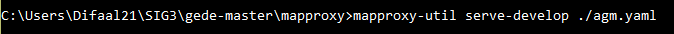
\includegraphics[width=12cm]{figures/Tugas5/1174076/1.png}
		\centering
		\caption{Run Mapproxy}
	\end{figure}
	
	\item Buka file basic.html pada folder leafletjs
    \hfill\break
    \begin{figure}[H]
		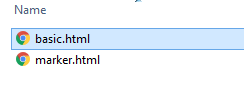
\includegraphics[width=12cm]{figures/Tugas5/1174076/2.png}
		\centering
		\caption{Open basic.html}
	\end{figure}
	
	\item Lalu buka file tersebut di browser, maka hasilnya akan seperti ini
    \hfill\break
    \begin{figure}[H]
		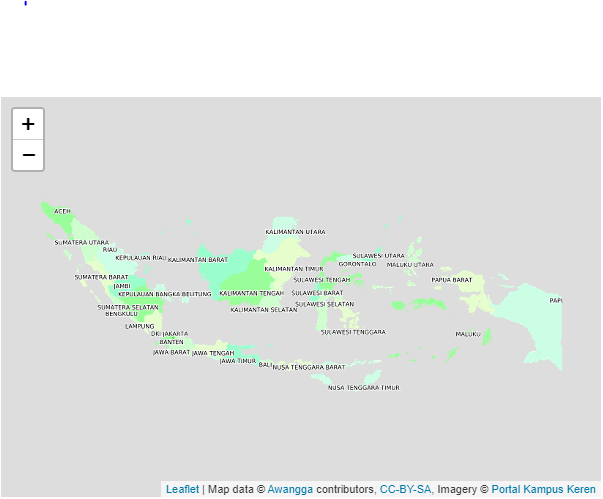
\includegraphics[width=12cm]{figures/Tugas5/1174076/3.png}
		\centering
		\caption{Hasil basic.html}
	\end{figure}
	
	\item Dengan leafletjs kita juga dapat menambahkan marker,circle, ataupun polygon dengan cara menggunakan seperti di gambar, contoh ini diambil
          dari file contoh kedua yaitu marker.html dari folder gede 
    \hfill\break
	
	\item Buka file marker.html
    \hfill\break
	\begin{figure}[H]
		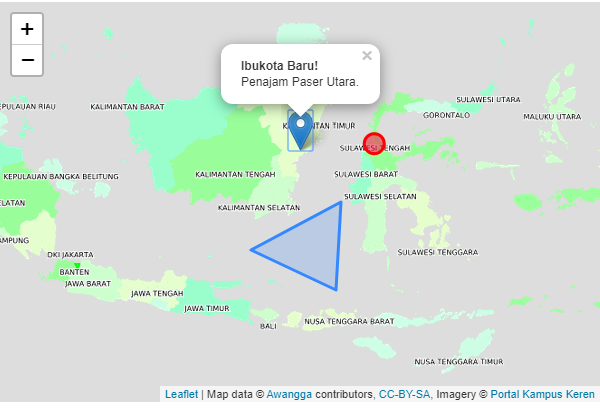
\includegraphics[width=12cm]{figures/Tugas5/1174076/4.png}
		\centering
		\caption{Hasil marker.html}
	\end{figure}
\end{enumerate}

\subsection{Link}
\url{https://youtu.be/xWDgij_GD_E}
  